\section{Monster Class Reference}
\label{classMonster}\index{Monster@{Monster}}
General class for any person, which can move, fight, communicate...  


{\tt \#include $<$monster.hpp$>$}

Inheritance diagram for Monster::\begin{figure}[H]
\begin{center}
\leavevmode
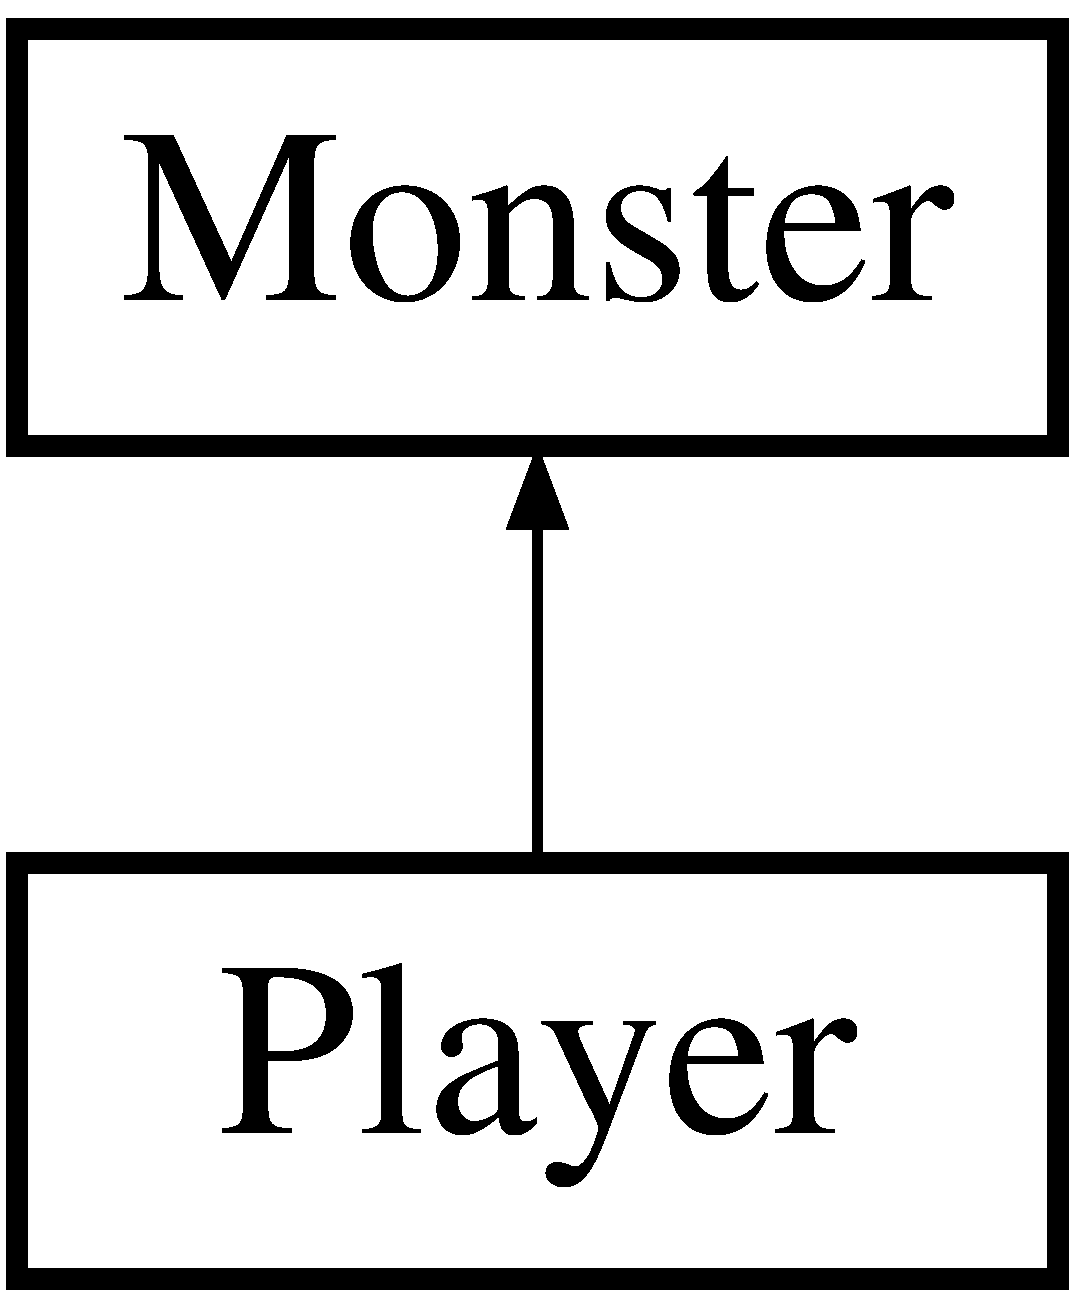
\includegraphics[height=2cm]{classMonster}
\end{center}
\end{figure}
\subsection*{Signals}
\begin{CompactItemize}
\item 
void {\bf map\-Changed} ()
\end{CompactItemize}
\subsection*{Public Member Functions}
\begin{CompactItemize}
\item 
{\bf Monster} ()
\item 
virtual {\bf $\sim$Monster} ()
\item 
void {\bf clear} ()
\item 
virtual void {\bf load} ({\bf Parser} \&parser)
\item 
virtual void {\bf save} (ofstream \&file) const 
\item 
virtual void {\bf random} (int {\bf monster\-Type})
\item 
void {\bf load\-Health\-State} ({\bf Parser} \&parser)
\item 
int {\bf get\-Monster\-Type} ()
\item 
virtual void {\bf reset\-Maximums} ()
\item 
void {\bf energy\-Move} ()
\item 
virtual void {\bf naturally\-Regenerate} ()
\item 
bool {\bf is\-Alive} ()
\item 
bool {\bf is\-Concious} ()
\item 
int {\bf chance} (double rating\-Diff)
\item 
int {\bf roll\-Dice} (int multiplier, int maximum)
\item 
int {\bf dv} () const 
\begin{CompactList}\small\item\em Defensive value. \item\end{CompactList}\item 
void {\bf melee\-Attack} ({\bf Monster} \&{\bf target})
\item 
void {\bf weapon\-Attack} ({\bf Monster} \&{\bf target}, {\bf Attack\-Descriptor} \&att\-Desc, QList$<$ int $>$ attack\-Skills)
\item 
bool {\bf can\-Equip\-As} (int item\-ID, int equip\-Slot) const 
\begin{CompactList}\small\item\em Tests whether monster is capable of equipping item into slot. \item\end{CompactList}\item 
void {\bf equip} (int item\-ID, int equip\-Slot)
\begin{CompactList}\small\item\em Equips monster with item. \item\end{CompactList}\item 
QPair$<$ bool, QString $>$ {\bf is\-Slot\-Equippable} (int equip\-Slot)
\begin{CompactList}\small\item\em Tests whether equip slot can be equipped. \item\end{CompactList}\item 
{\bf Attack\-Descriptor} {\bf unarmed\-Attack\-Descriptor} () const 
\begin{CompactList}\small\item\em Constructs and returns attack descriptor for unarmed fighting for this monster. \item\end{CompactList}\item 
int {\bf square\-Range\-To} ({\bf Monster} \&{\bf target})
\item 
{\bf Items\-List} {\bf take\-All\-Items} ()
\item 
void {\bf print} ()
\begin{CompactList}\small\item\em Prints monster name, level and attributes. \item\end{CompactList}\item 
bool {\bf increase\-Skill} (int skill, float value)
\item 
int {\bf skill\-Level} (int skill) const 
\begin{CompactList}\small\item\em Returns level of a skill. \item\end{CompactList}\item 
virtual bool {\bf is\-Monster} ()
\item 
QString {\bf get\-Map\-Name} () const 
\item 
void {\bf set\-Map\-Name} (const QString {\bf map\-Name})
\item 
int {\bf get\-Monster\-Type} () const 
\item 
void {\bf set\-Monster\-Type} (int type)
\item 
virtual bool {\bf teleport} (const QString \&{\bf map\-Name}, int {\bf x}, int {\bf y})
\begin{CompactList}\small\item\em Moves monster from it's current map to a map named {\tt map\-Name} at coordinates (x, y). \item\end{CompactList}\item 
virtual void {\bf move\-By} (int dx, int dy)
\item 
void {\bf ai\-Move} ()
\item 
virtual void {\bf damaged} ()
\item 
int {\bf get\-X} () const 
\item 
int {\bf get\-Y} () const 
\item 
void {\bf set\-X} (int {\bf x})
\item 
void {\bf set\-Y} (int {\bf y})
\item 
int {\bf get\-Hp} () const 
\item 
int {\bf get\-Fp} () const 
\item 
int {\bf get\-Mp} () const 
\item 
int {\bf get\-Max\-Hp} () const 
\item 
int {\bf get\-Max\-Fp} () const 
\item 
int {\bf get\-Max\-Mp} () const 
\item 
void {\bf finished\-Loading} ()
\end{CompactItemize}
\subsection*{Public Attributes}
\begin{CompactItemize}
\item 
QString {\bf name}
\item 
{\bf Items\-List} {\bf items}
\item 
QMap$<$ int, {\bf Item} $>$ {\bf equipment}
\item 
int {\bf energy}
\end{CompactItemize}
\subsection*{Protected Member Functions}
\begin{CompactItemize}
\item 
void {\bf p\-Save} (ofstream \&file, const char $\ast$padding\-Spaces) const 
\item 
void {\bf p\-Load} ({\bf Parser} \&parser)
\item 
void {\bf repaint} ()
\end{CompactItemize}
\subsection*{Protected Attributes}
\begin{CompactItemize}
\item 
QString {\bf map\-Name}
\item 
int {\bf x}
\item 
int {\bf y}
\item 
int {\bf monster\-Type}
\item 
int {\bf attributes} [9]
\item 
int {\bf maxhp}
\item 
int {\bf hp}
\item 
int {\bf maxfp}
\item 
int {\bf fp}
\item 
int {\bf maxmp}
\item 
int {\bf mp}
\item 
int {\bf hpfrac}
\item 
int {\bf fpfrac}
\item 
int {\bf mpfrac}
\item 
QMap$<$ int, {\bf Skill} $>$ {\bf skills}
\item 
{\bf Monster} $\ast$ {\bf target}
\item 
bool {\bf loaded}
\end{CompactItemize}


\subsection{Detailed Description}
General class for any person, which can move, fight, communicate... 



\subsection{Constructor \& Destructor Documentation}
\index{Monster@{Monster}!Monster@{Monster}}
\index{Monster@{Monster}!Monster@{Monster}}
\subsubsection{\setlength{\rightskip}{0pt plus 5cm}{\bf Monster} ()}\label{classMonster_a0}


\index{Monster@{Monster}!~Monster@{$\sim$Monster}}
\index{~Monster@{$\sim$Monster}!Monster@{Monster}}
\subsubsection{\setlength{\rightskip}{0pt plus 5cm}$\sim${\bf Monster} ()\hspace{0.3cm}{\tt  [virtual]}}\label{classMonster_a1}




\subsection{Member Function Documentation}
\index{Monster@{Monster}!aiMove@{aiMove}}
\index{aiMove@{aiMove}!Monster@{Monster}}
\subsubsection{\setlength{\rightskip}{0pt plus 5cm}void ai\-Move ()}\label{classMonster_a34}


\index{Monster@{Monster}!canEquipAs@{canEquipAs}}
\index{canEquipAs@{canEquipAs}!Monster@{Monster}}
\subsubsection{\setlength{\rightskip}{0pt plus 5cm}bool can\-Equip\-As (int {\em item\-ID}, int {\em equip\-Slot}) const}\label{classMonster_a18}


Tests whether monster is capable of equipping item into slot. 

Tests whether monster has enough stats, skills etc. to equip specified item into slot

\begin{Desc}
\item[Parameters:]
\begin{description}
\item[{\em item\-ID}]index of item to be equipped in {\bf Monster::items}{\rm (p.\,\pageref{classMonster_o1})}\item[{\em equip\-Slot}]equipment slot to be equipped to\end{description}
\end{Desc}
\begin{Desc}
\item[Returns:]whether monster is capable of equipping item into slot\end{Desc}
\index{Monster@{Monster}!chance@{chance}}
\index{chance@{chance}!Monster@{Monster}}
\subsubsection{\setlength{\rightskip}{0pt plus 5cm}int chance (double {\em rating\-Diff})}\label{classMonster_a13}


\index{Monster@{Monster}!clear@{clear}}
\index{clear@{clear}!Monster@{Monster}}
\subsubsection{\setlength{\rightskip}{0pt plus 5cm}void clear ()}\label{classMonster_a2}


\index{Monster@{Monster}!damaged@{damaged}}
\index{damaged@{damaged}!Monster@{Monster}}
\subsubsection{\setlength{\rightskip}{0pt plus 5cm}void damaged ()\hspace{0.3cm}{\tt  [virtual]}}\label{classMonster_a35}




Reimplemented in {\bf Player} {\rm (p.\,\pageref{classPlayer_a8})}.\index{Monster@{Monster}!dv@{dv}}
\index{dv@{dv}!Monster@{Monster}}
\subsubsection{\setlength{\rightskip}{0pt plus 5cm}int dv () const}\label{classMonster_a15}


Defensive value. 

Defensive value is used when calculating chance to hit this monster. Higher value means monster will be harder to hit. It depends on monster's Dexterity, combat skills and equipment

\begin{Desc}
\item[{\bf Todo}]dv from equipment\end{Desc}
\begin{Desc}
\item[Returns:]defensive value\end{Desc}
\index{Monster@{Monster}!energyMove@{energyMove}}
\index{energyMove@{energyMove}!Monster@{Monster}}
\subsubsection{\setlength{\rightskip}{0pt plus 5cm}void energy\-Move ()}\label{classMonster_a9}


\index{Monster@{Monster}!equip@{equip}}
\index{equip@{equip}!Monster@{Monster}}
\subsubsection{\setlength{\rightskip}{0pt plus 5cm}void equip (int {\em item\-ID}, int {\em equip\-Slot})}\label{classMonster_a19}


Equips monster with item. 

Equips monster with item whose index in inventory is {\tt item\-ID} into slot {\tt equip\-Slot} 

\begin{Desc}
\item[Parameters:]
\begin{description}
\item[{\em item\-ID}]index used to look for item in {\bf Monster::items}{\rm (p.\,\pageref{classMonster_o1})}. if {\tt item\-ID} is -1, slot is unequipped\item[{\em equip\-Slot}]equip slot to be equipped or unequipped\end{description}
\end{Desc}
\index{Monster@{Monster}!finishedLoading@{finishedLoading}}
\index{finishedLoading@{finishedLoading}!Monster@{Monster}}
\subsubsection{\setlength{\rightskip}{0pt plus 5cm}void finished\-Loading ()}\label{classMonster_a46}


\index{Monster@{Monster}!getFp@{getFp}}
\index{getFp@{getFp}!Monster@{Monster}}
\subsubsection{\setlength{\rightskip}{0pt plus 5cm}int get\-Fp () const}\label{classMonster_a41}


\index{Monster@{Monster}!getHp@{getHp}}
\index{getHp@{getHp}!Monster@{Monster}}
\subsubsection{\setlength{\rightskip}{0pt plus 5cm}int get\-Hp () const}\label{classMonster_a40}


\index{Monster@{Monster}!getMapName@{getMapName}}
\index{getMapName@{getMapName}!Monster@{Monster}}
\subsubsection{\setlength{\rightskip}{0pt plus 5cm}QString get\-Map\-Name () const}\label{classMonster_a28}


\index{Monster@{Monster}!getMaxFp@{getMaxFp}}
\index{getMaxFp@{getMaxFp}!Monster@{Monster}}
\subsubsection{\setlength{\rightskip}{0pt plus 5cm}int get\-Max\-Fp () const}\label{classMonster_a44}


\index{Monster@{Monster}!getMaxHp@{getMaxHp}}
\index{getMaxHp@{getMaxHp}!Monster@{Monster}}
\subsubsection{\setlength{\rightskip}{0pt plus 5cm}int get\-Max\-Hp () const}\label{classMonster_a43}


\index{Monster@{Monster}!getMaxMp@{getMaxMp}}
\index{getMaxMp@{getMaxMp}!Monster@{Monster}}
\subsubsection{\setlength{\rightskip}{0pt plus 5cm}int get\-Max\-Mp () const}\label{classMonster_a45}


\index{Monster@{Monster}!getMonsterType@{getMonsterType}}
\index{getMonsterType@{getMonsterType}!Monster@{Monster}}
\subsubsection{\setlength{\rightskip}{0pt plus 5cm}int get\-Monster\-Type () const}\label{classMonster_a30}


\index{Monster@{Monster}!getMonsterType@{getMonsterType}}
\index{getMonsterType@{getMonsterType}!Monster@{Monster}}
\subsubsection{\setlength{\rightskip}{0pt plus 5cm}int get\-Monster\-Type ()}\label{classMonster_a7}


\index{Monster@{Monster}!getMp@{getMp}}
\index{getMp@{getMp}!Monster@{Monster}}
\subsubsection{\setlength{\rightskip}{0pt plus 5cm}int get\-Mp () const}\label{classMonster_a42}


\index{Monster@{Monster}!getX@{getX}}
\index{getX@{getX}!Monster@{Monster}}
\subsubsection{\setlength{\rightskip}{0pt plus 5cm}int get\-X () const}\label{classMonster_a36}


\index{Monster@{Monster}!getY@{getY}}
\index{getY@{getY}!Monster@{Monster}}
\subsubsection{\setlength{\rightskip}{0pt plus 5cm}int get\-Y () const}\label{classMonster_a37}


\index{Monster@{Monster}!increaseSkill@{increaseSkill}}
\index{increaseSkill@{increaseSkill}!Monster@{Monster}}
\subsubsection{\setlength{\rightskip}{0pt plus 5cm}bool increase\-Skill (int {\em skill}, float {\em value})}\label{classMonster_a25}


\index{Monster@{Monster}!isAlive@{isAlive}}
\index{isAlive@{isAlive}!Monster@{Monster}}
\subsubsection{\setlength{\rightskip}{0pt plus 5cm}bool is\-Alive ()}\label{classMonster_a11}


\index{Monster@{Monster}!isConcious@{isConcious}}
\index{isConcious@{isConcious}!Monster@{Monster}}
\subsubsection{\setlength{\rightskip}{0pt plus 5cm}bool is\-Concious ()}\label{classMonster_a12}


\index{Monster@{Monster}!isMonster@{isMonster}}
\index{isMonster@{isMonster}!Monster@{Monster}}
\subsubsection{\setlength{\rightskip}{0pt plus 5cm}bool is\-Monster ()\hspace{0.3cm}{\tt  [virtual]}}\label{classMonster_a27}




Reimplemented in {\bf Player} {\rm (p.\,\pageref{classPlayer_a2})}.\index{Monster@{Monster}!isSlotEquippable@{isSlotEquippable}}
\index{isSlotEquippable@{isSlotEquippable}!Monster@{Monster}}
\subsubsection{\setlength{\rightskip}{0pt plus 5cm}QPair$<$ bool, QString $>$ is\-Slot\-Equippable (int {\em equip\-Slot})}\label{classMonster_a20}


Tests whether equip slot can be equipped. 

If, for example, monster is carrying something with both hands, then hand and offhand slots can't be used.

\begin{Desc}
\item[{\bf Todo}]restriction to equip rings when gloves are equipped\end{Desc}
\begin{Desc}
\item[Parameters:]
\begin{description}
\item[{\em equip\-Slot}]slot to be equipped\end{description}
\end{Desc}
\begin{Desc}
\item[Returns:]a pair of {\tt boolean} value and a {\tt QString} message. {\tt boolean} value will be {\bf true}, if slot is equippable, else it will be {\bf false} and message will contain human-readable {\tt QString} with reason\end{Desc}
\index{Monster@{Monster}!load@{load}}
\index{load@{load}!Monster@{Monster}}
\subsubsection{\setlength{\rightskip}{0pt plus 5cm}void load ({\bf Parser} \& {\em parser})\hspace{0.3cm}{\tt  [virtual]}}\label{classMonster_a3}




Reimplemented in {\bf Player} {\rm (p.\,\pageref{classPlayer_a0})}.\index{Monster@{Monster}!loadHealthState@{loadHealthState}}
\index{loadHealthState@{loadHealthState}!Monster@{Monster}}
\subsubsection{\setlength{\rightskip}{0pt plus 5cm}void load\-Health\-State ({\bf Parser} \& {\em parser})}\label{classMonster_a6}


\index{Monster@{Monster}!mapChanged@{mapChanged}}
\index{mapChanged@{mapChanged}!Monster@{Monster}}
\subsubsection{\setlength{\rightskip}{0pt plus 5cm}void map\-Changed ()\hspace{0.3cm}{\tt  [signal]}}\label{classMonster_l0}


\index{Monster@{Monster}!meleeAttack@{meleeAttack}}
\index{meleeAttack@{meleeAttack}!Monster@{Monster}}
\subsubsection{\setlength{\rightskip}{0pt plus 5cm}void melee\-Attack ({\bf Monster} \& {\em target})}\label{classMonster_a16}


\index{Monster@{Monster}!moveBy@{moveBy}}
\index{moveBy@{moveBy}!Monster@{Monster}}
\subsubsection{\setlength{\rightskip}{0pt plus 5cm}void move\-By (int {\em dx}, int {\em dy})\hspace{0.3cm}{\tt  [virtual]}}\label{classMonster_a33}




Reimplemented in {\bf Player} {\rm (p.\,\pageref{classPlayer_a4})}.\index{Monster@{Monster}!naturallyRegenerate@{naturallyRegenerate}}
\index{naturallyRegenerate@{naturallyRegenerate}!Monster@{Monster}}
\subsubsection{\setlength{\rightskip}{0pt plus 5cm}void naturally\-Regenerate ()\hspace{0.3cm}{\tt  [virtual]}}\label{classMonster_a10}




Reimplemented in {\bf Player} {\rm (p.\,\pageref{classPlayer_a7})}.\index{Monster@{Monster}!pLoad@{pLoad}}
\index{pLoad@{pLoad}!Monster@{Monster}}
\subsubsection{\setlength{\rightskip}{0pt plus 5cm}void p\-Load ({\bf Parser} \& {\em parser})\hspace{0.3cm}{\tt  [protected]}}\label{classMonster_b1}


\index{Monster@{Monster}!print@{print}}
\index{print@{print}!Monster@{Monster}}
\subsubsection{\setlength{\rightskip}{0pt plus 5cm}void print ()}\label{classMonster_a24}


Prints monster name, level and attributes. 

\index{Monster@{Monster}!pSave@{pSave}}
\index{pSave@{pSave}!Monster@{Monster}}
\subsubsection{\setlength{\rightskip}{0pt plus 5cm}void p\-Save (ofstream \& {\em file}, const char $\ast$ {\em padding\-Spaces}) const\hspace{0.3cm}{\tt  [protected]}}\label{classMonster_b0}


\index{Monster@{Monster}!random@{random}}
\index{random@{random}!Monster@{Monster}}
\subsubsection{\setlength{\rightskip}{0pt plus 5cm}void random (int {\em monster\-Type})\hspace{0.3cm}{\tt  [virtual]}}\label{classMonster_a5}




Reimplemented in {\bf Player} {\rm (p.\,\pageref{classPlayer_a5})}.\index{Monster@{Monster}!repaint@{repaint}}
\index{repaint@{repaint}!Monster@{Monster}}
\subsubsection{\setlength{\rightskip}{0pt plus 5cm}void repaint ()\hspace{0.3cm}{\tt  [protected]}}\label{classMonster_b2}


\index{Monster@{Monster}!resetMaximums@{resetMaximums}}
\index{resetMaximums@{resetMaximums}!Monster@{Monster}}
\subsubsection{\setlength{\rightskip}{0pt plus 5cm}void reset\-Maximums ()\hspace{0.3cm}{\tt  [virtual]}}\label{classMonster_a8}




Reimplemented in {\bf Player} {\rm (p.\,\pageref{classPlayer_a6})}.\index{Monster@{Monster}!rollDice@{rollDice}}
\index{rollDice@{rollDice}!Monster@{Monster}}
\subsubsection{\setlength{\rightskip}{0pt plus 5cm}int roll\-Dice (int {\em multiplier}, int {\em maximum})}\label{classMonster_a14}


\index{Monster@{Monster}!save@{save}}
\index{save@{save}!Monster@{Monster}}
\subsubsection{\setlength{\rightskip}{0pt plus 5cm}void save (ofstream \& {\em file}) const\hspace{0.3cm}{\tt  [virtual]}}\label{classMonster_a4}




Reimplemented in {\bf Player} {\rm (p.\,\pageref{classPlayer_a1})}.\index{Monster@{Monster}!setMapName@{setMapName}}
\index{setMapName@{setMapName}!Monster@{Monster}}
\subsubsection{\setlength{\rightskip}{0pt plus 5cm}void set\-Map\-Name (const QString {\em map\-Name})}\label{classMonster_a29}


\index{Monster@{Monster}!setMonsterType@{setMonsterType}}
\index{setMonsterType@{setMonsterType}!Monster@{Monster}}
\subsubsection{\setlength{\rightskip}{0pt plus 5cm}void set\-Monster\-Type (int {\em type})}\label{classMonster_a31}


\index{Monster@{Monster}!setX@{setX}}
\index{setX@{setX}!Monster@{Monster}}
\subsubsection{\setlength{\rightskip}{0pt plus 5cm}void set\-X (int {\em x})}\label{classMonster_a38}


\index{Monster@{Monster}!setY@{setY}}
\index{setY@{setY}!Monster@{Monster}}
\subsubsection{\setlength{\rightskip}{0pt plus 5cm}void set\-Y (int {\em y})}\label{classMonster_a39}


\index{Monster@{Monster}!skillLevel@{skillLevel}}
\index{skillLevel@{skillLevel}!Monster@{Monster}}
\subsubsection{\setlength{\rightskip}{0pt plus 5cm}int skill\-Level (int {\em skill}) const}\label{classMonster_a26}


Returns level of a skill. 

\index{Monster@{Monster}!squareRangeTo@{squareRangeTo}}
\index{squareRangeTo@{squareRangeTo}!Monster@{Monster}}
\subsubsection{\setlength{\rightskip}{0pt plus 5cm}int square\-Range\-To ({\bf Monster} \& {\em target})}\label{classMonster_a22}


\index{Monster@{Monster}!takeAllItems@{takeAllItems}}
\index{takeAllItems@{takeAllItems}!Monster@{Monster}}
\subsubsection{\setlength{\rightskip}{0pt plus 5cm}{\bf Items\-List} take\-All\-Items ()}\label{classMonster_a23}


\index{Monster@{Monster}!teleport@{teleport}}
\index{teleport@{teleport}!Monster@{Monster}}
\subsubsection{\setlength{\rightskip}{0pt plus 5cm}bool teleport (const QString \& {\em map\-Name}, int {\em x}, int {\em y})\hspace{0.3cm}{\tt  [virtual]}}\label{classMonster_a32}


Moves monster from it's current map to a map named {\tt map\-Name} at coordinates (x, y). 

Doesn't check whether it can be moved here. \begin{Desc}
\item[Returns:]false, if such map or square does not exist\end{Desc}


Reimplemented in {\bf Player} {\rm (p.\,\pageref{classPlayer_a3})}.\index{Monster@{Monster}!unarmedAttackDescriptor@{unarmedAttackDescriptor}}
\index{unarmedAttackDescriptor@{unarmedAttackDescriptor}!Monster@{Monster}}
\subsubsection{\setlength{\rightskip}{0pt plus 5cm}{\bf Attack\-Descriptor} unarmed\-Attack\-Descriptor () const}\label{classMonster_a21}


Constructs and returns attack descriptor for unarmed fighting for this monster. 

\index{Monster@{Monster}!weaponAttack@{weaponAttack}}
\index{weaponAttack@{weaponAttack}!Monster@{Monster}}
\subsubsection{\setlength{\rightskip}{0pt plus 5cm}void weapon\-Attack ({\bf Monster} \& {\em target}, {\bf Attack\-Descriptor} \& {\em att\-Desc}, QList$<$ int $>$ {\em attack\-Skills})}\label{classMonster_a17}




\subsection{Member Data Documentation}
\index{Monster@{Monster}!attributes@{attributes}}
\index{attributes@{attributes}!Monster@{Monster}}
\subsubsection{\setlength{\rightskip}{0pt plus 5cm}int {\bf attributes}[9]\hspace{0.3cm}{\tt  [protected]}}\label{classMonster_p4}


\index{Monster@{Monster}!energy@{energy}}
\index{energy@{energy}!Monster@{Monster}}
\subsubsection{\setlength{\rightskip}{0pt plus 5cm}int {\bf energy}}\label{classMonster_o3}


\index{Monster@{Monster}!equipment@{equipment}}
\index{equipment@{equipment}!Monster@{Monster}}
\subsubsection{\setlength{\rightskip}{0pt plus 5cm}QMap$<$int,{\bf Item}$>$ {\bf equipment}}\label{classMonster_o2}


\index{Monster@{Monster}!fp@{fp}}
\index{fp@{fp}!Monster@{Monster}}
\subsubsection{\setlength{\rightskip}{0pt plus 5cm}int {\bf fp}\hspace{0.3cm}{\tt  [protected]}}\label{classMonster_p8}


\index{Monster@{Monster}!fpfrac@{fpfrac}}
\index{fpfrac@{fpfrac}!Monster@{Monster}}
\subsubsection{\setlength{\rightskip}{0pt plus 5cm}int {\bf fpfrac}\hspace{0.3cm}{\tt  [protected]}}\label{classMonster_p12}


\index{Monster@{Monster}!hp@{hp}}
\index{hp@{hp}!Monster@{Monster}}
\subsubsection{\setlength{\rightskip}{0pt plus 5cm}int {\bf hp}\hspace{0.3cm}{\tt  [protected]}}\label{classMonster_p6}


\index{Monster@{Monster}!hpfrac@{hpfrac}}
\index{hpfrac@{hpfrac}!Monster@{Monster}}
\subsubsection{\setlength{\rightskip}{0pt plus 5cm}int {\bf hpfrac}\hspace{0.3cm}{\tt  [protected]}}\label{classMonster_p11}


\index{Monster@{Monster}!items@{items}}
\index{items@{items}!Monster@{Monster}}
\subsubsection{\setlength{\rightskip}{0pt plus 5cm}{\bf Items\-List} {\bf items}}\label{classMonster_o1}


\index{Monster@{Monster}!loaded@{loaded}}
\index{loaded@{loaded}!Monster@{Monster}}
\subsubsection{\setlength{\rightskip}{0pt plus 5cm}bool {\bf loaded}\hspace{0.3cm}{\tt  [protected]}}\label{classMonster_p16}


\index{Monster@{Monster}!mapName@{mapName}}
\index{mapName@{mapName}!Monster@{Monster}}
\subsubsection{\setlength{\rightskip}{0pt plus 5cm}QString {\bf map\-Name}\hspace{0.3cm}{\tt  [protected]}}\label{classMonster_p0}


\index{Monster@{Monster}!maxfp@{maxfp}}
\index{maxfp@{maxfp}!Monster@{Monster}}
\subsubsection{\setlength{\rightskip}{0pt plus 5cm}int {\bf maxfp}\hspace{0.3cm}{\tt  [protected]}}\label{classMonster_p7}


\index{Monster@{Monster}!maxhp@{maxhp}}
\index{maxhp@{maxhp}!Monster@{Monster}}
\subsubsection{\setlength{\rightskip}{0pt plus 5cm}int {\bf maxhp}\hspace{0.3cm}{\tt  [protected]}}\label{classMonster_p5}


\index{Monster@{Monster}!maxmp@{maxmp}}
\index{maxmp@{maxmp}!Monster@{Monster}}
\subsubsection{\setlength{\rightskip}{0pt plus 5cm}int {\bf maxmp}\hspace{0.3cm}{\tt  [protected]}}\label{classMonster_p9}


\index{Monster@{Monster}!monsterType@{monsterType}}
\index{monsterType@{monsterType}!Monster@{Monster}}
\subsubsection{\setlength{\rightskip}{0pt plus 5cm}int {\bf monster\-Type}\hspace{0.3cm}{\tt  [protected]}}\label{classMonster_p3}


\index{Monster@{Monster}!mp@{mp}}
\index{mp@{mp}!Monster@{Monster}}
\subsubsection{\setlength{\rightskip}{0pt plus 5cm}int {\bf mp}\hspace{0.3cm}{\tt  [protected]}}\label{classMonster_p10}


\index{Monster@{Monster}!mpfrac@{mpfrac}}
\index{mpfrac@{mpfrac}!Monster@{Monster}}
\subsubsection{\setlength{\rightskip}{0pt plus 5cm}int {\bf mpfrac}\hspace{0.3cm}{\tt  [protected]}}\label{classMonster_p13}


\index{Monster@{Monster}!name@{name}}
\index{name@{name}!Monster@{Monster}}
\subsubsection{\setlength{\rightskip}{0pt plus 5cm}QString {\bf name}}\label{classMonster_o0}


\index{Monster@{Monster}!skills@{skills}}
\index{skills@{skills}!Monster@{Monster}}
\subsubsection{\setlength{\rightskip}{0pt plus 5cm}QMap$<$int, {\bf Skill}$>$ {\bf skills}\hspace{0.3cm}{\tt  [protected]}}\label{classMonster_p14}


\index{Monster@{Monster}!target@{target}}
\index{target@{target}!Monster@{Monster}}
\subsubsection{\setlength{\rightskip}{0pt plus 5cm}{\bf Monster}$\ast$ {\bf target}\hspace{0.3cm}{\tt  [protected]}}\label{classMonster_p15}


\index{Monster@{Monster}!x@{x}}
\index{x@{x}!Monster@{Monster}}
\subsubsection{\setlength{\rightskip}{0pt plus 5cm}int {\bf x}\hspace{0.3cm}{\tt  [protected]}}\label{classMonster_p1}


\index{Monster@{Monster}!y@{y}}
\index{y@{y}!Monster@{Monster}}
\subsubsection{\setlength{\rightskip}{0pt plus 5cm}int {\bf y}\hspace{0.3cm}{\tt  [protected]}}\label{classMonster_p2}




The documentation for this class was generated from the following files:\begin{CompactItemize}
\item 
{\bf monster.hpp}\item 
{\bf monster.cpp}\end{CompactItemize}
